% ====================================================================
% VİZE RAPOR ŞABLONU – Türk Masalları Derlemesi Web Sayfası
% --------------------------------------------------------------------
% DERLEME: Overleaf'te Menu > Compiler > XeLaTeX (pdfLaTeX de çalışır).
%
% KURALLAR (şablonu kullanmadan önce okuyun):
%  1. Bölüm başlıklarını SİLMEYİN ve sırasını DEĞİŞTİRMEYİN.
%  2. [KÖŞELİ PARANTEZ] içindeki ve gri renkli açıklama metinlerini
%     kendi bilgilerinizle değiştirin; açıklama metinlerini silin.
%  3. MEBİS'e YALNIZCA bu raporun PDF'ini yükleyin.
%     ZIP ve HTML dosyası YÜKLEMEYİN. Tüm kontroller GitHub'dan yapılır.
%  4. Kapaktaki GitHub ve YouTube bağlantıları doğru ve tıklanabilir
%     olmalıdır. Teslimden önce PDF'teki bağlantılara tıklayıp deneyin.
%  5. Haftalık katkı tablosundaki görseller için resim dosyalarını
%     (hafta1.png, hafta2.png, ...) Overleaf projesine yükleyin.
%     Dosya adlarında boşluk ve Türkçe karakter kullanmayın.
%     Resim yoksa tabloda "görsel ekleyin" kutusu görünür.
%  6. Yapay zekâ kullandıysanız Bölüm 5'i doldurun.
% ====================================================================
\documentclass[12pt,a4paper]{article}

\usepackage{iftex}
\ifPDFTeX
  \usepackage[T1]{fontenc}
  \usepackage[utf8]{inputenc}
\else
  \usepackage{fontspec}
\fi
\usepackage[turkish]{babel}
\usepackage[margin=2.4cm]{geometry}
\usepackage{setspace}
\usepackage{graphicx}
\usepackage{booktabs}
\usepackage{longtable}
\usepackage{array}
\usepackage{colortbl}
\usepackage{xcolor}
\usepackage{enumitem}
\usepackage{listings}
\usepackage{amssymb}
\usepackage{caption}
\usepackage{fancyhdr}
\setlength{\headheight}{15pt}
\usepackage{hyperref}

\onehalfspacing
\setlength{\parindent}{0pt}
\setlength{\parskip}{6pt}
\setlist{itemsep=2pt, topsep=4pt}
\hypersetup{colorlinks=true, linkcolor=blue!50!black, urlcolor=blue!50!black}

\definecolor{ana}{HTML}{14325C}
\definecolor{acik}{HTML}{EEF2F8}

\lstset{basicstyle=\ttfamily\small, backgroundcolor=\color{acik},
  frame=single, rulecolor=\color{ana}, breaklines=true,
  columns=fullflexible, keepspaces=true, showstringspaces=false}

\pagestyle{fancy}
\fancyhf{}
\fancyhead[L]{Bir Varmış}
\fancyhead[R]{Vize Raporu}
\fancyfoot[C]{\thepage}

% ---------- Yardımcı komutlar ----------
% Gri açıklama metni (silinecek yönergeler için)
\newcommand{\aciklama}[1]{{\color{gray}\itshape (#1)}}

% Haftalık tablo görseli: dosya yoksa "görsel ekleyin" kutusu çıkar
\newcommand{\haftagorsel}[1]{%
  \IfFileExists{#1}{%
    \includegraphics[width=\linewidth,height=4.2cm,keepaspectratio]{#1}%
  }{%
    \fbox{\parbox[c][2.6cm][c]{\dimexpr\linewidth-2\fboxsep-2\fboxrule\relax}{%
      \centering\small\color{gray} Ekran görüntüsü / görsel ekleyin\\ \texttt{#1}}}%
  }%
}
% Haftalık katılım kutuları (işaretlemek için $\square$ yerine $\boxtimes$ yazın)
\newcommand{\katilimkutulari}{\par\vspace{3pt}\small $\square$ Ders içinde katılım sergiledim\par $\square$ Telafi yaptım}

% Ek görsel: dosya yoksa hiçbir şey göstermez
\newcommand{\haftaek}[1]{%
  \IfFileExists{#1}{\\[4pt]\includegraphics[width=\linewidth,height=4.2cm,keepaspectratio]{#1}}{}%
}

% ---------- Kapak bilgileri ----------
\newcommand{\universite}{Medipol Üniversitesi / Görsel İletişim Tasarımı}
\newcommand{\dersadi}{Programlamaya Giriş}
\newcommand{\hocaadi}{Meral Şentürk}
\newcommand{\ogrenciadi}{[AD SOYAD]}
\newcommand{\ogrencino}{[ÖĞRENCİ NUMARASI]}
\newcommand{\projeadi}{Bir Varmış}
% Bağlantıları tam adres olarak yazın (https:// ile başlayarak)
\newcommand{\githublink}{\url{https://github.com/KULLANICI-ADI/DEPO-ADI}}
\newcommand{\youtubelink}{\url{https://www.youtube.com/watch?v=VIDEO-KIMLIGI}}

\begin{document}

% ====================================================================
% KAPAK
% ====================================================================
\begin{titlepage}
\centering
\vspace*{1cm}
{\large \universite \par}
\vspace{1.8cm}
{\Huge\bfseries\color{ana} \projeadi \par}
\vspace{0.4cm}
{\Large Türk Masalları Derlemesi Web Sayfası \par}
{\large Vize Raporu \par}
\vspace{0.4cm}
{\small\color{red!65!black} ÇALIŞMA TASLAĞI: Öğrenci bilgileri, bağlantılar,
haftalık katkılar ve kişisel değerlendirmeler tamamlanmalıdır.\par}
\vspace{1.8cm}
{\large \textbf{Ders:} \dersadi \par}
{\large \textbf{Öğretim Üyesi:} \hocaadi \par}
\vspace{1.2cm}
{\large \textbf{Hazırlayan:} \ogrenciadi \par}
{\large \textbf{Öğrenci No:} \ogrencino \par}
\vspace{1.8cm}
\fbox{\parbox{0.88\linewidth}{\centering\vspace{6pt}
{\large\bfseries Proje Bağlantıları}\\[8pt]
\textbf{GitHub deposu:}\\ \githublink \\[8pt]
\textbf{YouTube sunum videosu:}\\ \youtubelink
\vspace{6pt}}}
\vfill
{\large \today \par}
\end{titlepage}

\tableofcontents
\newpage

% ====================================================================
\section{Giriş}
% ====================================================================


\subsection{Proje Özeti}
Bir Varmış, Türk halk anlatılarından seçilen yayımlanmış sekiz masal metnini
bir araya getiren bir okuma sayfasıdır. Amaç, kültürel çağrışımları olan sade bir
arayüzde masallara kolay ulaşılmasını sağlamaktır. Sayfa tek bir HTML dosyasından
oluşur; CSS ve JavaScript kodları dosyanın içinde yer alır. Masal arama, masal
seçme, önceki ve sonraki masala geçme ile yazı boyutu ayarı JavaScript ile çalışır.
Harici font, görsel veya kütüphane kullanılmadığı için okuma işlevleri internet
bağlantısı gerektirmez. Bu raporda seçimler, tasarım gerekçeleri ve kodun işleyişi
anlatılmaktadır. Metinler kaynaklarından alınmış ve kaynak bilgileri sayfada belirtilmiştir.

\subsection{Gereksinimlerin Karşılanması}
\begin{center}
\rowcolors{2}{acik}{white}
\begin{tabular}{@{}p{8.2cm}c@{}}
\toprule
\rowcolor{ana}\textcolor{white}{\textbf{Gereksinim}} & \textcolor{white}{\textbf{Durum}} \\
\midrule
Masal sayısı 8--12 arasında (8 masal)         & $\boxtimes$ \\
Tek HTML dosyası                                    & $\boxtimes$ \\
Stil kodları içsel (\texttt{<style>} içinde)        & $\boxtimes$ \\
Betik kodları içsel (\texttt{<script>} içinde)      & $\boxtimes$ \\
İnternetsiz açılıp çalışıyor                        & $\square$ \\
JavaScript sayfada anlamlı bir işlev görüyor        & $\boxtimes$ \\
Masal metinleri kendi cümlelerimle yazıldı          & $\square$ \\
Sayfa telefonda da düzgün görünüyor                 & $\square$ \\
\bottomrule
\end{tabular}
\end{center}


% ====================================================================

Dosyanın internet kapalıyken açılması ve gerçek telefonda kontrolü sonrasında
ilgili kutular işaretlenmelidir. Bu sürümde masallar kaynak metin olarak
aktarıldığından kendi cümleleriyle yazma kutusu işaretlenmemiştir.
Şablondaki bu koşul için öğrencinin öğretim üyesiyle kaynak metin kullanımını
netleştirmesi gerekir; özgün metin olduğu iddia edilmemektedir.

\section{Masalların Seçimi}
% ====================================================================


Sekiz masal, yayımlanmış Türkçe metinlerden seçilmiştir. Altı anonim anlatı
Vikikaynak sayfalarından; Keloğlan ve Tembel Ahmet ise Ziya Gökalp'in
Altın Işık eserinin erişime açık e-kitap önizlemesinden alınmıştır. Kaynak
metinler yeniden yazılmamış, yalnızca paragraf düzeni uyarlanmıştır.
Yöresel söyleyişler ve kaynaklardaki yazım korunmuştur. Vikikaynak katkıcılarına
atıf verilmiş, CC BY-SA 4.0 lisans bilgisi kaynak bağlantılarıyla birlikte sunulmuştur.

\begin{longtable}{@{}cp{4cm}p{3cm}p{5.4cm}@{}}
\toprule
\textbf{No} & \textbf{Masal} & \textbf{Tür} & \textbf{Seçilme nedeni} \\
\midrule
\endhead
1 & Keloğlan ve Padişah & Halk masalı & Hayvanlara yapılan iyiliklerin karşılığını konu alması. \\
2 & Tembel Ahmet & Halk masalı & Çalışma, değişim ve cesaret temalarını birleştirmesi. \\
3 & Keloğlan & Halk masalı & Ziya Gökalp'in yayımlanmış masal anlatımını örneklemesi. \\
4 & Tembel Kız & Halk masalı & Emek ve sorumluluk temasını kısa bir anlatıyla işlemesi. \\
5 & Karanan ile Tilki & Halk masalı & Zincirleme anlatı yapısı ve dürüstlük temasını içermesi. \\
6 & Külden Eşek & Halk masalı & Dev ve sihirli eşek motifleriyle halk anlatısını örneklemesi. \\
7 & On iki gardaş meseli & Yöresel masal & Kıbrıs ağzını ve kardeşlik çevresindeki çatışmaları göstermesi. \\
8 & İncircinin dediği & Yöresel masal & Aile içi iletişimi yöresel bir anlatımla ele alması. \\
\bottomrule
\end{longtable}

% ====================================================================
\section{Tasarım Kararları}
% ====================================================================


\subsection{Konuya Uygunluk}
Beyaz zemin, okuma alanını ferah tutar. Bordo masal başlıklarında; turkuaz ana düğmede, üst kenar çizgisinde, seçili masalda ve gezinme ayrıntılarında kullanılır. Bu renkler masal temasını ölçülü biçimde destekler. Turkuaz, Türk rengi olarak anılması ve adının Türklerle bağlantısı nedeniyle kültürel bir çağrışım kurmak için seçilmiştir. Fransızca turquoise sözcüğü, Türk anlamındaki eski turcois sıfatından gelir; bu adlandırma taşın Türkiye üzerinden tanınmasıyla ilişkilidir. Bu etimolojik bağlantı tasarım tercihinin gerekçesidir \cite{renk}. Kilim geometrisinden esinlenen SVG motif,
sayfa için basit çizgilerle oluşturulmuştur; belirli bir tarihî motifi aynen
temsil ettiği iddia edilmemektedir. Büyük süslemeler yerine okuma metni öne çıkar.
Hazır web sitesi teması veya şablon paketi kullanılmamıştır.

\subsection{Renk Paleti ve Yazı Tipi}
\begin{center}
\rowcolors{2}{acik}{white}
\begin{tabular}{@{}llp{6.4cm}@{}}
\toprule
\rowcolor{ana}\textcolor{white}{\textbf{Ad}} & \textcolor{white}{\textbf{Kod}} & \textcolor{white}{\textbf{Nerede / neden kullandınız?}} \\
\midrule
Bordo & \texttt{\#713344} & Ana başlıklar ve masal metninin ilk harfi. \\
Turkuaz & \texttt{\#147D86} & Ana düğme, üst çizgi, seçili masal, motif ve gezinme. \\
Beyaz & \texttt{\#FFFFFF} & Ferah okuma zemini. \\
Açık gri & \texttt{\#F7F8F6} & Hafif liste arka planı. \\
Georgia / Segoe UI & -- & Masal ve başlıklarda serif; menü ve düğmelerde sade sistem yazısı. \\
\bottomrule
\end{tabular}
\end{center}

\subsection{Okunabilirlik, Gezinme ve Duyarlı Tasarım}
\begin{itemize}
  \item \textbf{Okunabilirlik:} Metin 19 piksel Georgia ile başlar, 17--25 piksel arasında ayarlanabilir. Satır aralığı 1.9, satır uzunluğu en fazla 65ch değerindedir. Koyu metin beyaz zeminde kullanılır.
  \item \textbf{Gezinme:} Soldaki başlık listesinden seçim yapılır. Arama, başlık ve tema sözcüklerini Türkçe harf kurallarıyla süzer. Alt düğmeler sekiz masalın tamamındaki sırayı izler; arama yalnızca listeyi süzer.
  \item \textbf{Duyarlı tasarım:} 760 piksel ve altında liste ile okuma alanı alt alta gelir. Liste iki sütuna dönüşür ve büyük süsleme gizlenir. Gerçek cihaz doğrulaması öğrenci tarafından tamamlanmalıdır.
  \item \textbf{Tutarlılık:} Aynı renk değişkenleri, çizgiler, boşluk ölçüleri ve düğme biçimleri tüm sayfada tekrar edilir.
\end{itemize}

\subsection{Ekran Görüntüleri}
\begin{figure}[htbp]
\centering
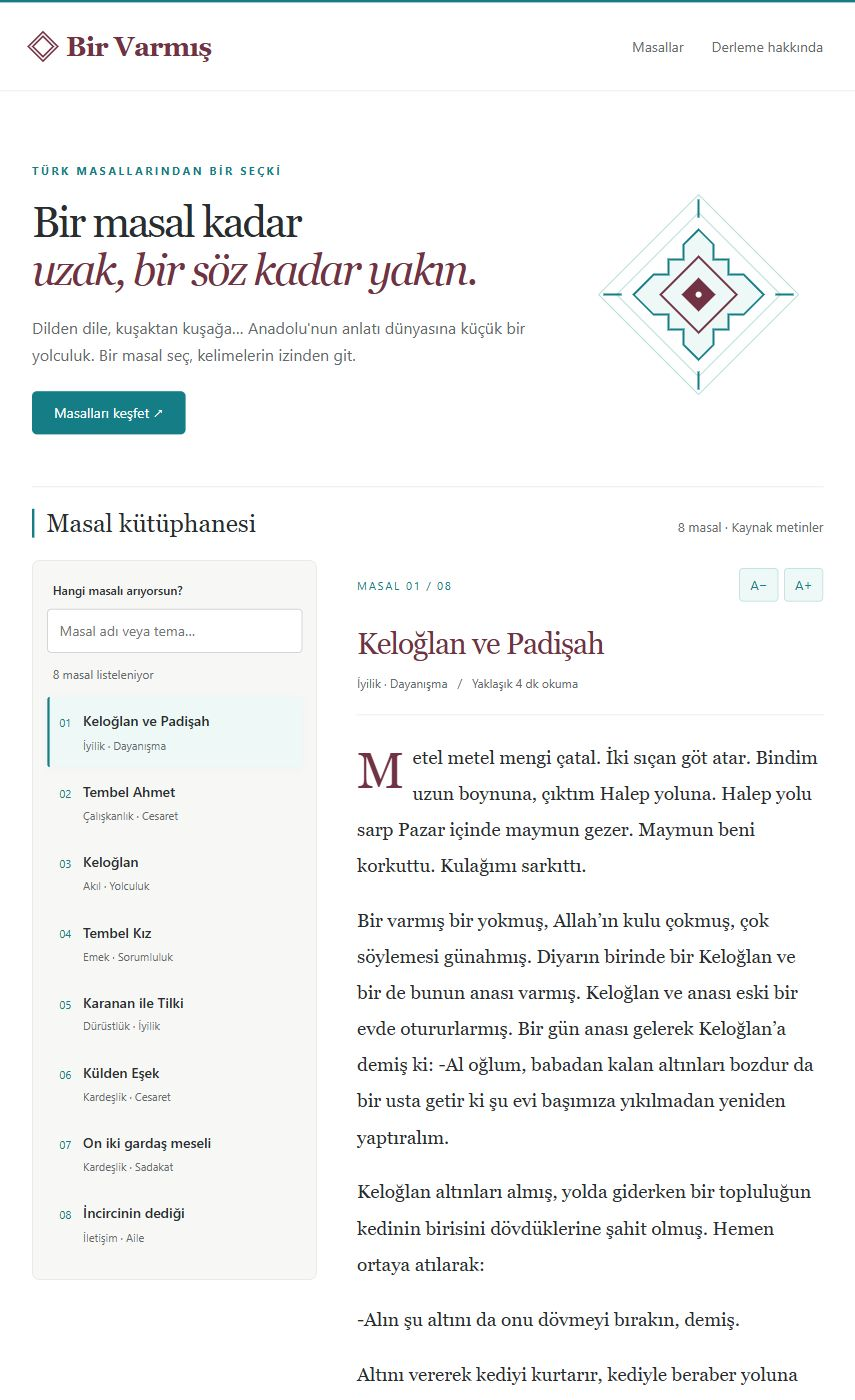
\includegraphics[width=\linewidth]{ekran-masaustu.png}
\caption{Tarayıcıda masaüstü görünümü.}
\end{figure}
\begin{figure}[htbp]
\centering
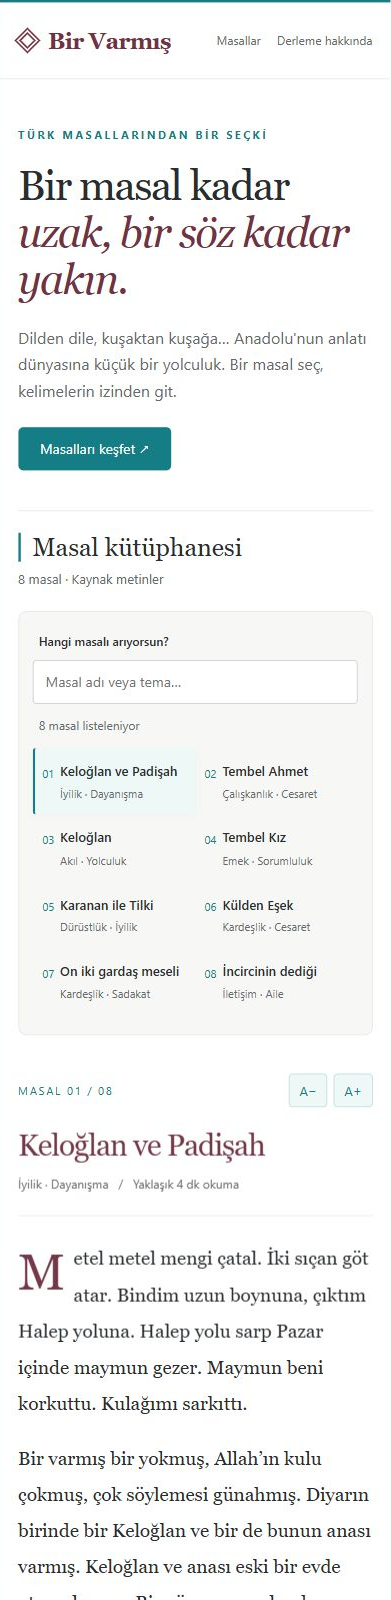
\includegraphics[width=0.42\textwidth,height=13cm,keepaspectratio]{ekran-mobil.png}
\caption{390 piksel genişliğindeki tarayıcı çerçevesinde mobil yerleşim. Gerçek telefon testi değildir.}
\end{figure}

\section{Gerçekleştirme}
% ====================================================================


\subsection{HTML Yapısı}
Üst bilgi header, ana içerik main, tematik bölümler section, masal seçimi aside,
masallar article, alt bilgi footer etiketleriyle kurulur. Sekiz masal doğrudan
HTML içinde tutulur. Her masalın başlığı, tema bilgisi, paragrafları ve kaynak
adı bulunur. hidden özelliği, seçilmeyen masalları gizler. Seçim için button,
sayfa içi gezinme için a etiketleri kullanılır.

\subsection{İçsel CSS}
CSS, head bölümündeki style etiketi içindedir. Renkler :root altında değişken
olarak tanımlanır. Ana yerleşim CSS Grid ile 285 piksel liste ve kalan genişliği
kullanan okuma alanına ayrılır. Küçük ekran kuralı bu düzeni tek sütuna çevirir.
Seçili düğmenin sol kenarı turkuaz, zemini açık turkuaz olur. Kısa belirme geçişi kullanılır; hareketi
azaltma tercihi olan kullanıcılarda animasyon kaldırılır.

\begin{lstlisting}[caption={İçsel CSS'ten önemli bir bölüm}]
.kutuphane {
  display: grid;
  grid-template-columns: 285px 1fr;
  gap: 40px;
}
@media (max-width: 760px) {
  .kutuphane { grid-template-columns: 1fr; }
}
\end{lstlisting}

\subsection{İçsel JavaScript}
Masal metinleri JavaScript dizisinde değil, HTML article elemanlarında tutulur.
querySelectorAll ile masallar ve seçim düğmeleri bulunur; Array.from ile dizilere
çevrilir. secili değişkeni mevcut masalın sırasını tutar. masalAc fonksiyonu
forEach ile yalnızca seçilen masalın hidden değerini false yapar ve düğmelerin
aria-pressed değerini günceller. Arama olayında toLocaleLowerCase('tr-TR') ile
Türkçe büyük ve küçük harfler eşleştirilir, includes ile başlık ve tema içinde
aranır. yaziAyarla fonksiyonu boyutu 17--25 piksel arasında sınırlar. Tıklama
ve yazma olayları addEventListener ile bağlanır. Harici dosya veya veri isteği
yoktur; kaynak bağlantısı yalnızca kullanıcı onu açarsa internet gerektirir.

\begin{lstlisting}[caption={İçsel JavaScript'ten önemli bir bölüm}]
masallar.forEach((masal, i) => {
  masal.hidden = i !== sira;
});
\end{lstlisting}

\subsection{Sayfanın Özellikleri}
\begin{itemize}
\item Sekiz masal arasında seçim ve sıra ile gezinme.
\item Masal başlığı ve temasına göre anlık arama; boş sonuç açıklaması.
\item Beş kademeli yazı boyutu; alt ve üst sınırda düğmenin kapanması.
\item Klavye odağı, anlamlı başlıklar ve okuma alanına atlama bağlantısı.
\item Duyarlı yerleşim, hareket azaltma tercihi ve internetsiz kullanım.
\end{itemize}


% ====================================================================
\section{Yapay Zekâ Kullanımı}
% ====================================================================


\begin{longtable}{@{}p{2.6cm}p{3.6cm}p{4.2cm}p{3.4cm}@{}}
\toprule
\textbf{Araç} & \textbf{Ne için kullandınız?} & \textbf{İstem (prompt) özeti} & \textbf{Sayfada nerede?} \\
\midrule
\endhead
OpenAI Codex & Kod ve rapor düzenleme desteği & Sade bir masal okuma sayfası hazırlama & HTML, CSS, JavaScript ve rapor taslağı. \\
\bottomrule
\end{longtable}

\subsection{Anladığım ve Kendim Yaptığım Kısımlar}
[Bu alanı öğrenci kendi deneyimine göre doldurmalıdır. Önce ayrı kod rehberindeki
alıştırmaları uygulayın. Hangi rengi, metni veya davranışı değiştirdiğinizi ve
ne öğrendiğinizi somut örneklerle anlatın. Yapılmamış bir çalışma yazmayın.]

% ====================================================================
\section{Haftalık Katkılar}
% ====================================================================
\aciklama{Her hafta ders içinde yaptığınız çalışmayı kısaca yazın (2--4 cümle). Hangi
özelliği eklediğinizi ya da neyi düzelttiğinizi belirtin ve ilgili commit mesajını
ya da bağlantısını ``Commit'' satırına yazın. Her satıra ekran görüntüsü ekleyin:
resimleri \texttt{hafta1.png}, \texttt{hafta2.png}, \ldots{} adıyla Overleaf
projesine yükleyin. Aynı haftaya ikinci bir görsel eklemek için
\texttt{hafta1b.png} gibi bir dosya yükleyin; kendiliğinden görünür.
Her haftanın altındaki kutulardan o hafta için geçerli olanı $\boxtimes$ ile
işaretleyin: dersin kendisinde katılım gösterdiyseniz ``Ders içinde katılım
sergiledim'', o haftayı sonradan tamamladıysanız ``Telafi yaptım''. Telafi
yaptıysanız yapılan çalışmanın metninde bunu açıkça belirtin.}

\begin{longtable}{@{}>{\raggedright\arraybackslash}p{1.7cm}%
                    >{\raggedright\arraybackslash}p{6.4cm}%
                    >{\centering\arraybackslash}p{6cm}@{}}
\toprule
\rowcolor{ana}\textcolor{white}{\textbf{Hafta}} & \textcolor{white}{\textbf{Yapılan çalışma}} & \textcolor{white}{\textbf{Görsel}} \\
\midrule
\endfirsthead
\toprule
\rowcolor{ana}\textcolor{white}{\textbf{Hafta}} & \textcolor{white}{\textbf{Yapılan çalışma}} & \textcolor{white}{\textbf{Görsel}} \\
\midrule
\endhead
\bottomrule
\endfoot

\textbf{1. hafta}\newline [tarih] &
[Bu hafta yaptığınız çalışma.]\newline \textbf{Commit:} [mesaj veya bağlantı]\katilimkutulari &
\haftagorsel{hafta1.png}\haftaek{hafta1b.png} \\
\midrule
\textbf{2. hafta}\newline [tarih] &
[Bu hafta yaptığınız çalışma.]\newline \textbf{Commit:} [mesaj veya bağlantı]\katilimkutulari &
\haftagorsel{hafta2.png}\haftaek{hafta2b.png} \\
\midrule
\textbf{3. hafta}\newline [tarih] &
[Bu hafta yaptığınız çalışma.]\newline \textbf{Commit:} [mesaj veya bağlantı]\katilimkutulari &
\haftagorsel{hafta3.png}\haftaek{hafta3b.png} \\
\midrule
\textbf{4. hafta}\newline [tarih] &
[Bu hafta yaptığınız çalışma.]\newline \textbf{Commit:} [mesaj veya bağlantı]\katilimkutulari &
\haftagorsel{hafta4.png}\haftaek{hafta4b.png} \\
\midrule
\textbf{5. hafta}\newline [tarih] &
[Bu hafta yaptığınız çalışma.]\newline \textbf{Commit:} [mesaj veya bağlantı]\katilimkutulari &
\haftagorsel{hafta5.png}\haftaek{hafta5b.png} \\
\midrule
\textbf{6. hafta}\newline [tarih] &
[Bu hafta yaptığınız çalışma.]\newline \textbf{Commit:} [mesaj veya bağlantı]\katilimkutulari &
\haftagorsel{hafta6.png}\haftaek{hafta6b.png} \\
\midrule
\textbf{7. hafta}\newline [tarih] &
[Bu hafta yaptığınız çalışma.]\newline \textbf{Commit:} [mesaj veya bağlantı]\katilimkutulari &
\haftagorsel{hafta7.png}\haftaek{hafta7b.png} \\
\midrule
\textbf{8. hafta}\newline [tarih] &
[Bu hafta yaptığınız çalışma.]\newline \textbf{Commit:} [mesaj veya bağlantı]\katilimkutulari &
\haftagorsel{hafta8.png}\haftaek{hafta8b.png} \\
\end{longtable}

% ====================================================================
\section{Test ve Değerlendirme}
Tarayıcıda yapılan yardımcı doğrulama: sekiz masalın seçimi, Türkçe arama,
boş sonuç, gezinme uçları ve yazı boyutu sınırları kontrol edilmiştir.
390 piksel genişliğinde aynı kökenli bir iframe içinde mobil yerleşim
incelenmiştir. Gerçek telefon ve çevrimdışı dosya açma denemeleri öğrenci
tarafından da yapılmalıdır; bu taslak öğrencinin yapmış olduğu testleri
varsaymaz. Aşağıdaki tablo kendi denemelerinden sonra doldurulmalıdır.

% ====================================================================


\begin{center}
\rowcolors{2}{acik}{white}
\begin{tabular}{@{}p{6cm}p{3.4cm}p{3.4cm}@{}}
\toprule
\rowcolor{ana}\textcolor{white}{\textbf{Özellik}} & \textcolor{white}{\textbf{Bilgisayar}} & \textcolor{white}{\textbf{Telefon}} \\
\midrule
\relax[Özellik 1] & [Çalışıyor / Sorun var] & [Çalışıyor / Sorun var] \\
\relax[Özellik 2] & [Çalışıyor / Sorun var] & [Çalışıyor / Sorun var] \\
\relax[Özellik 3] & [Çalışıyor / Sorun var] & [Çalışıyor / Sorun var] \\
\bottomrule
\end{tabular}
\end{center}

\textbf{Denenen tarayıcılar:} [Chrome, Firefox, Edge, Safari vb.]

% ====================================================================
\section{Sunum Videosu}
% ====================================================================
\begin{center}
\begin{tabular}{@{}ll@{}}
\textbf{Video süresi:} & [dakika:saniye] \quad  \\
\textbf{Görünürlük:} & [Listelenmemiş / Herkese açık] \\
\textbf{Bağlantı:} & \youtubelink \\
\end{tabular}
\end{center}

\subsection{Video Kontrol Listesi}

\begin{itemize}[label={}]
  \item $\square$ Süre 12--18 dakika aralığında.
  \item $\square$ Sunum boyunca kameram açık, yüzüm görünüyor.
  \item $\square$ Görünürlük \textbf{Listelenmemiş} (ya da Herkese açık); \textbf{Özel} değil.
  \item $\square$ Bağlantıyı gizli pencerede açtım, video oynuyor.
  \item $\square$ YouTube videoyu işlemeyi bitirdi.
  \item $\square$ Videoyu baştan sona izledim; ses ve kamera tüm sunumda var.
  \item $\square$ Kapaktaki bağlantı ile bu bölümdeki bağlantı aynı.
\end{itemize}

% ====================================================================
\section{Sonuç ve Kendi Değerlendirmem}
% ====================================================================


[Öğrencinin kendi değerlendirmesi: HTML, CSS ve JavaScript ilişkisinden ne
öğrendiniz? Kodu anlatırken hangi kısımda zorlandınız? Kaynak metinleri nasıl seçip
doğruladınız? Yaptığınız denemeler ve sonraki geliştirme fikrinizle birlikte
6--10 cümle yazın.]

% ====================================================================
\section{Kaynakça}
% ====================================================================


\begin{thebibliography}{99}
\bibitem{masal1} Anonim / Vikikaynak katkıcıları. \emph{Keloğlan ve Padişah}. \url{https://tr.wikisource.org/wiki/Kelo%C4%9Flan_ve_Padi%C5%9Fah}. Erişim: 6 Kasım 2026.
\bibitem{masal2} Ziya Gökalp, Altın Işık. \emph{Tembel Ahmet}. \url{https://litres-tr.com/book/ziya-gokalp/altin-isik-69428596/read/}. Erişim: 6 Kasım 2026.
\bibitem{masal3} Ziya Gökalp, Altın Işık. \emph{Keloğlan}. \url{https://litres-tr.com/book/ziya-gokalp/altin-isik-69428596/read/}. Erişim: 6 Kasım 2026.
\bibitem{masal4} Anonim / Vikikaynak katkıcıları. \emph{Tembel Kız}. \url{https://tr.wikisource.org/wiki/Tembel_K%C4%B1z}. Erişim: 6 Kasım 2026.
\bibitem{masal5} Anonim / Vikikaynak katkıcıları. \emph{Karanan ile Tilki}. \url{https://tr.wikisource.org/wiki/Karanan_ile_Tilki}. Erişim: 6 Kasım 2026.
\bibitem{masal6} Anonim / Vikikaynak katkıcıları. \emph{Külden Eşek}. \url{https://tr.wikisource.org/wiki/K%C3%BClden_E%C5%9Fek}. Erişim: 6 Kasım 2026.
\bibitem{masal7} Anonim / Vikikaynak katkıcıları. \emph{On iki gardaş meseli}. \url{https://tr.wikisource.org/wiki/On_iki_garda%C5%9F_meseli}. Erişim: 6 Kasım 2026.
\bibitem{masal8} Anonim / Vikikaynak katkıcıları. \emph{İncircinin dediği}. \url{https://tr.wikisource.org/wiki/%C4%B0ncircinin_dedi%C4%9Fi}. Erişim: 6 Kasım 2026.
\bibitem{ders} Meral Şentürk. \emph{Programlamaya Giriş -- Vize Bilgilendirme,
2026--2027 Güz} ve dersin vize raporu şablonu. Kullanıcı tarafından sağlanan ders belgeleri.
\bibitem{renk} Académie française. \emph{Turquoise}, Dictionnaire de l'Académie française, 9. baskı. \url{https://www.dictionnaire-academie.fr/article/A9T2745}. Erişim: 6 Kasım 2026.
\end{thebibliography}

% ====================================================================
\appendix
\section{Teslim Kontrol Listesi}
% ====================================================================

\begin{itemize}[label={}]
  \item $\square$ MEBİS'e \textbf{yalnızca bu raporun PDF'ini} yükleyeceğim. ZIP ve HTML dosyası yüklemeyeceğim.
  \item $\square$ PDF dosya adı \texttt{OgrenciNo\_AdSoyad\_vize.pdf} biçiminde.
  \item $\square$ Kapaktaki GitHub ve YouTube bağlantıları doğru; PDF'te tıklayıp denedim.
  \item $\square$ GitHub deposunda web sayfası (tek \texttt{.html}), rapor PDF'i, \texttt{.tex} kaynakları ve \texttt{README.md} var.
  \item $\square$ GitHub deposu \textbf{herkese açık} (ya da öğretim üyesine erişim verdim).
  \item $\square$ Çalışmamın son hâli teslim saatinden \textbf{önce} depoya gönderildi (sonraki commitler değerlendirilmez).
  \item $\square$ Sayfa içsel CSS ve içsel JavaScript kullanıyor, harici dosya gerektirmiyor.
  \item $\square$ Hazır taslak kullanmadım; yapay zekâ kullandıysam Bölüm 5'i doldurdum.
  \item $\square$ Çalışmanın mantığını sunumda anlatabilirim.
\end{itemize}

\end{document}